\begin{frame}{Scalability definitions}
  \begin{columns}
    \begin{column}{0.5\textwidth}
      {\large Strong scalability}
      \begin{itemize}
      \item Fixed problem size
      \item execution time $T$ inversely proportional to number of processors $p$
      \end{itemize}
    \end{column}
    \begin{column}{0.5\textwidth}
      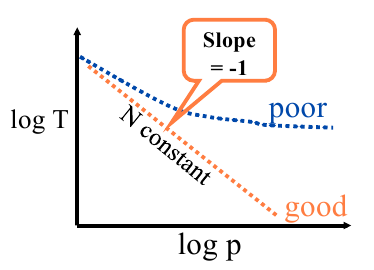
\includegraphics[width=\textwidth]{figures/KeyesStrongScaling.png}
    \end{column}
  \end{columns}
  \begin{columns}
    \begin{column}{0.5\textwidth}
      {\large Weak scalability}
      \begin{itemize}
      \item Fixed problem size per processor
      \item execution time constant as problem size increases
      \end{itemize}
    \end{column}
    \begin{column}{0.5\textwidth}
      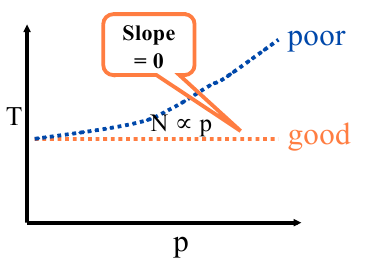
\includegraphics[width=\textwidth]{figures/KeyesWeakScaling.png}
    \end{column}
  \end{columns}
\end{frame}
